\documentclass{standalone}
\usepackage{tikz}
\usetikzlibrary{shapes,arrows,positioning,calc,patterns}

\begin{document}
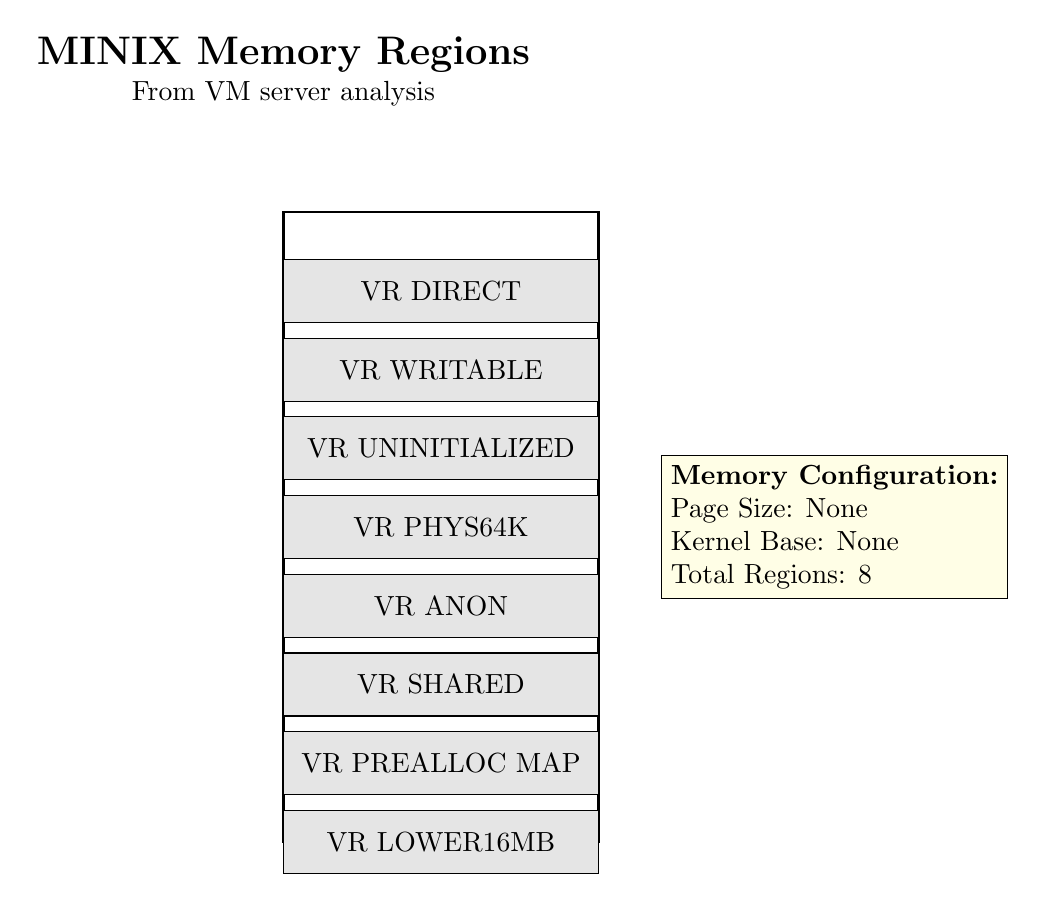
\begin{tikzpicture}[
    region/.style={rectangle, draw=black, minimum width=4cm, minimum height=0.8cm},
    arrow/.style={->, >=stealth}
]

% Title
\node[font=\Large\bfseries] at (0, 10) {MINIX Memory Regions};
\node[font=\normalsize] at (0, 9.5) {From VM server analysis};

% Memory layout
\draw[thick] (0, 0) rectangle (4, 8);

\node[region, fill=gray!20] at (2, 7) {VR DIRECT};
\node[region, fill=gray!20] at (2, 6.0) {VR WRITABLE};
\node[region, fill=gray!20] at (2, 5.0) {VR UNINITIALIZED};
\node[region, fill=gray!20] at (2, 4.0) {VR PHYS64K};
\node[region, fill=gray!20] at (2, 3.0) {VR ANON};
\node[region, fill=gray!20] at (2, 2.0) {VR SHARED};
\node[region, fill=gray!20] at (2, 1.0) {VR PREALLOC MAP};
\node[region, fill=gray!20] at (2, 0.0) {VR LOWER16MB};

% Memory Constants
\node[draw=black, fill=yellow!10, align=left] at (7, 4) {
\textbf{Memory Configuration:}\\
Page Size: None\\
Kernel Base: None\\
Total Regions: 8
};

\end{tikzpicture}
\end{document}